\section{Evaluation}
% 评估
\label{sec:eval}

Our evaluation addresses two research questions:
% 我们的评估围绕两个研究问题展开：

\begin{itemize}[leftmargin=*]
  \item \textbf{RQ1 (Policy Expressibility and Benefits):} Can AI agents safely express GPU resource-management policies through \sys---including policies from published state-of-the-art systems---and do those policies improve performance?
  % RQ1（策略可表达性与收益）：AI 智能体能否通过 gpubpf 安全地表达 GPU 资源管理策略——包括已发表最先进系统的策略——这些策略能否提升性能？
  \item \textbf{RQ2 (Mechanism Cost):} What does the \sys{} mechanism cost, in hook and observability overhead and in executing the same policy through \sys{}?
  % RQ2（机制代价）：gpubpf 机制的代价有多大——包括钩子与可观测开销，以及通过 gpubpf 执行同一策略的代价？
\end{itemize}

We answer RQ1 in \S\ref{sec:rq1} through policy microbenchmarks, agent-driven case studies on realistic workloads, multi-tenant settings, and comparisons with native implementations of published policies. \S\ref{sec:rq2-cost} answers RQ2.
% 我们在 \S\ref{sec:rq1} 通过策略微基准、真实负载上的智能体驱动案例研究、多租户场景，以及与已发表策略的原生实现的比较回答 RQ1；\S\ref{sec:rq2-cost} 回答 RQ2。

\subsection{Methodology and Setup}
% 方法论与实验设置

We evaluate \sys on two machines: Server~A with Intel Core Ultra~9 285K (24 cores), 128~GB DDR5 RAM, and NVIDIA RTX~5090 GPU; Server~B with dual Intel Gold 6138 (80 cores), 256~GB RAM, and NVIDIA P40 GPU.
% 我们在两台机器上评估 gpubpf：服务器 A 配备 Intel Core Ultra 9 285K（24 核）、128 GB DDR5 内存和 NVIDIA RTX 5090 GPU；服务器 B 配备双路 Intel Gold 6138（80 核）、256 GB 内存和 NVIDIA P40 GPU。
Unless otherwise specified, experiments run on Server~A, averaging 10 trials using geometric mean.
% 除非另有说明，实验均在服务器 A 上进行，每项结果取 10 次试验的几何平均值。
We compare \sys{} against three classes of baselines: (1) driver defaults (UVM LRU/FIFO eviction, native GPU scheduler), (2) application-level hints (\texttt{cudaMemAdvise}), and (3) framework-managed policies (e.g., llama.cpp \texttt{ncmoe}, vLLM CPU offload, LMCache) where applicable.
% 我们将 gpubpf 与三类基线对比：(1) 驱动默认行为（UVM LRU/FIFO 驱逐、原生 GPU 调度器），(2) 应用层提示（\texttt{cudaMemAdvise}），以及 (3) 框架管理的策略（如 llama.cpp 的 \texttt{ncmoe}、vLLM CPU offload、LMCache，在适用处）。
The comparisons in \S\ref{sec:policy-mechanism} additionally evaluate policies from published research systems: MoE-Infinity~\cite{xue2025moeinfinity}, XSched~\cite{shen2025xsched}, GPREEMPT~\cite{fan2025gpreempt}, Expert Buffering~\cite{huang2023towards}, FineMoE~\cite{yu2026finemoe}, Hummingbird~\cite{hu2026hummingbird}, and POD-Attention~\cite{kamath2025pod}; each pairs a native policy implementation with a \sys{} port.
% \S\ref{sec:policy-mechanism} 进一步评估 MoE-Infinity、XSched、GPREEMPT、Expert Buffering、FineMoE、Hummingbird 和 POD-Attention 等已发表系统的策略；每组配对原生策略实现和 \sys{} 移植版。
We use PyTorch (version 2.9.0) and vLLM (version 0.11.0) with custom allocators, llama.cpp (version 7101), and Faiss (version 1.13.0) with UVM build config.
% 我们使用 PyTorch（版本 2.9.0）和 vLLM（版本 0.11.0，配自定义分配器）、llama.cpp（版本 7101）以及采用 UVM 构建配置的 Faiss（版本 1.13.0）。
All tests with \sys policies require no application modifications.
% 所有使用 gpubpf 策略的测试均无需修改应用。

\begin{figure}
\centering

\includegraphics[width=\columnwidth]{img/results-raw/clc/microbench_combined.pdf}
\caption{Single-tenant policy evaluation (normalized speedup, higher is better): (a) memory prefetch policies on vector-add; (b) block scheduling policies on GEMM.}
% 单租户策略评估（归一化加速比，越高越好）：(a) vector-add 上的内存预取策略；(b) GEMM 上的块调度策略。
\label{fig:clc-policies}

\end{figure}

\subsection{RQ1: Policy Expressibility and Benefits}
% RQ1：策略可表达性与收益
\label{sec:rq1}

\subsubsection{Single-Tenant Memory and Scheduling Policies}
% 单租户内存与调度策略
\label{sec:rq1-micro}

\paragraph{Memory Prefetch Policies.}
% 内存预取策略。
We evaluate host-device prefetch coordination using a vector-add GPU kernel~\cite{nvidia_cuda_samples} with stride access pattern and 40GB working set (1.25$\times$ oversubscription).
% 我们使用具有步长访问模式、40GB 工作集（1.25× 超订）的 vector-add GPU 内核~\cite{nvidia_cuda_samples}评估主机—设备预取协同。
Device-side L2 prefetch instructions (\texttt{prefetch.\allowbreak{}global.\allowbreak{}L2}) trigger non-blocking page faults, while host-side callbacks extend prefetching to additional pages.
% 设备端 L2 预取指令（\texttt{prefetch.\allowbreak{}global.\allowbreak{}L2}）触发非阻塞缺页，而主机端回调将预取扩展到更多页面。
As shown in \Cref{fig:clc-policies}a, device-only prefetch at thread entry achieves 1.34$\times$ speedup while combined host-device stride-based eBPF prefetch achieves 1.77$\times$.
% 如 \Cref{fig:clc-policies}a 所示，仅设备端预取在线程入口处取得 1.34× 加速，而主机—设备协同的步长式 eBPF 预取达到 1.77×。
However, sequential prefetch degrades performance by 8\% due to pattern mismatch.
% 然而，顺序预取因模式不匹配导致性能下降 8\%。

\paragraph{Single-Tenant Block Scheduler.}
% 单租户块调度器。
We apply a \sys-based thread block scheduler to workloads with load imbalance.
% 我们将基于 gpubpf 的线程块调度器应用于存在负载不均衡的工作负载。
Using cluster-style launch where persistent worker blocks pull work units through a policy decision, we evaluate three policies: FixedWork (static block assignment, no scheduler), Greedy (always-steal), and LatencyBudget (workload-aware with per-block time limits).
% 采用集群式启动，由持久工作块根据策略决策 拉取工作单元，我们评估三种策略：FixedWork（静态块分配，无调度器）、Greedy（总是窃取）和 LatencyBudget（感知负载、带每块时间限制的策略）。
\Cref{fig:clc-policies}b compares these policies across two GEMM workloads.
% \Cref{fig:clc-policies}b 在两种 GEMM 工作负载上对比了这些策略。
Under moderate imbalance, both Greedy and LatencyBudget reduce latency by $\sim$11\%.
% 在中等不均衡下，Greedy 和 LatencyBudget 均将延迟降低约 11\%。
Under heavy-tail workloads where 10\% of blocks perform 100--200$\times$ more work, Greedy increases latency by 20\% due to contention on heavy blocks.
% 在 10\% 的块承担 100--200× 更多工作量的重尾负载下，Greedy 因对重块的竞争使延迟增加 20\%。
LatencyBudget, which caps per-block stealing time, matches fixed-work baseline.
% LatencyBudget 限制了每块的窃取时间，与固定分配基线持平。
This highlights \sys's programmability: different workloads require different scheduling strategies.
% 这凸显了 gpubpf 的可编程性：不同工作负载需要不同的调度策略。

\subsubsection{Agent-Driven Policy Exploration Case Studies}
% 智能体驱动的策略探索案例研究
\label{sec:rq1-agent}

We provided an AI coding agent (Claude Code with Opus 4.5) with \sys{}'s eBPF interfaces; the agent autonomously generated all policy logic without human review or guidance, while humans authored only the initial framework and benchmark harness.
% 我们向一个 AI 编程智能体（Claude Code，Opus 4.5）提供 gpubpf 的 eBPF 接口；智能体在无人审阅或指导的情况下自主生成了全部策略逻辑，人类只编写初始框架和基准测试工具。
All 59 policies evaluated were produced via a fully automated generate-test-iterate loop.
% 评估的全部 59 个策略均由完全自动化的“生成—测试—迭代”循环产出。
We conclude with four case studies showing performance gains and the exploration process.
% 最后我们通过四个案例研究展示性能收益与探索过程。

\paragraph{Expert Offloading (llama.cpp GPT-OSS-120B).}
% 专家卸载（llama.cpp GPT-OSS-120B）。
We evaluate \sys on GPT-OSS-120B MXFP4 MoE (59~GB) in llama.cpp on RTX 5090 (32~GB), requiring 1.84$\times$ oversubscription.
% 我们在 RTX 5090（32 GB）上的 llama.cpp 中评估 GPT-OSS-120B MXFP4 MoE（59 GB），需要 1.84× 超订。
We compare five configurations: framework-managed CPU offloading (\texttt{ncmoe=\allowbreak{}32/64}), default UVM, UVM with application-level hints (\texttt{cuda\-Mem\-Advise}), and \sys with eBPF-based host-device prefetching (\S\ref{sec:design-interfaces}).
% 我们对比五种配置：框架管理的 CPU 卸载（\texttt{ncmoe=\allowbreak{}32/64}）、默认 UVM、带应用层提示的 UVM（\texttt{cuda\-Mem\-Advise}），以及采用基于 eBPF 的主机—设备预取的 gpubpf（\S\ref{sec:design-interfaces}）。
\Cref{fig:llama-expert-offload} shows prefill and decode throughput.
% \Cref{fig:llama-expert-offload} 给出了预填充与解码吞吐量。
For decode (memory-bound), \sys achieves \textbf{1.76$\times$ speedup} over application-tuned UVM hints (\texttt{cuda\-Mem\-Advise}) and 4.8$\times$ over framework offloading (\texttt{ncmoe=64}).
% 对于解码（内存受限），gpubpf 相比经应用调优的 UVM 提示（\texttt{cuda\-Mem\-Advise}）取得 \textbf{1.76× 加速}，相比框架卸载（\texttt{ncmoe=64}）取得 4.8× 加速。
These hints improve decode over default UVM but require application modification and degrade prefill by 40\%; \sys outperforms hints on decode while preserving prefill within 4\% of default UVM, without application changes.
% 这些提示相比默认 UVM 改善了解码，但需要修改应用，并使预填充性能下降 40\%；gpubpf 在解码上优于提示，同时将预填充保持在默认 UVM 的 4\% 以内，且无需修改应用。
For prefill (compute-bound), framework offloading (\texttt{ncmoe=32}) achieves 13\% higher prefill throughput than \sys{}, but decode dominates end-to-end latency, so the decode improvement outweighs the prefill gap.%\arq{I don't understand the final data point. what has 13\% higher throughput? The graphed performance of UVM eBPF looks like it has worse performance compared to the alternatives. BTW---its very weird that none of the bars in Figure 8 are labeled "\sys"--I think that UVM eBPF is supposed to be that configuration but it does not make a lot of sense.}
% 对于预填充（计算受限），框架卸载（\texttt{ncmoe=32}）比 gpubpf 的预填充吞吐量高 13\%，但解码主导端到端延迟，因此解码的改善超过了预填充的差距。

The agent arrived at the final policy through iterative exploration: sequential prefetch degraded decode throughput due to mismatch with MoE stride patterns (consistent with the 8\% degradation in \Cref{fig:clc-policies}a), leading to stride-based prefetch aligned with regular weight layout within each expert layer.
% 智能体通过迭代探索得出最终策略：顺序预取因与 MoE 步长模式不匹配而降低了解码吞吐量（与 \Cref{fig:clc-policies}a 中 8\% 的下降一致），于是改为与各专家层内规则权重布局对齐的步长预取。
Device-side eBPF tracing of per-warp memory accesses revealed that expert activations follow predictable stride sequences and identified frequently-accessed shared layers.
% 对每 warp 内存访问的设备端 eBPF 追踪表明，专家激活遵循可预测的步长序列，并识别出被频繁访问的共享层。
For eviction, the agent tested FIFO ordering before converging on LFU, which retains frequently-accessed shared layers while evicting cold expert pages.
% 在驱逐方面，智能体先测试 FIFO 顺序，最终收敛到 LFU——它保留被频繁访问的共享层，同时驱逐冷的专家页面。
The final policy combines device-side access observation, host-side stride prefetch, and LFU eviction (\S\ref{sec:design-interfaces}).
% 最终策略结合了设备端访问观测、主机端步长预取和 LFU 驱逐（\S\ref{sec:design-interfaces}）。

% \xiangyu{Are those hints easy to find in many scenarios? Maybe we should clarify it. Otherwise, it seems that \sys{} uses some tricks to win the competition.}

\begin{figure}
\centering

\includegraphics[width=\columnwidth]{img/results-raw/llama.cpp/llama_uvm_combined_color.pdf}

\caption{Prefill and decode throughput for GPT-OSS-120B MoE on llama.cpp.}
% llama.cpp 上 GPT-OSS-120B MoE 的预填充与解码吞吐量。
\label{fig:llama-expert-offload}

\end{figure}

\paragraph{KV-cache Offloading (vLLM Qwen-30B MoE).}
% KV-cache 卸载（vLLM Qwen-30B MoE）。
We evaluate \sys on the Qwen-30B FP8 MoE model ($\approx$30GB) on RTX 5090 (32GB).
% 我们在 RTX 5090（32GB）上评估 Qwen-30B FP8 MoE 模型（约 30GB）。
The model nearly fills GPU VRAM, so the default no-offload configuration OOMs under load.
% 该模型几乎占满 GPU 显存，因此默认的不卸载配置在负载下会 OOM。
We stress KV-cache growth by sending 100 concurrent requests from ShareGPT~\cite{sharegpt} (single-round, no prefix caching), resulting in 36--40GB total footprint ($\approx$60K tokens KV-cache).
% 我们通过发送来自 ShareGPT~\cite{sharegpt} 的 100 个并发请求（单轮、无前缀缓存）施加 KV-cache 增长压力，总占用达 36--40GB（约 60K token 的 KV-cache）。
Existing solutions offload KV-cache or experts but not both; UVM attempts on-demand migration of both, leading to thrashing.
% 现有方案只卸载 KV-cache 或专家权重之一；UVM 则尝试对二者按需迁移，导致抖动。
We compare vLLM's CPU-offload mode (\texttt{--cpu-offload-gb 8}) against \sys with UVM and a sequential prefetch policy.
% 我们将 vLLM 的 CPU 卸载模式（\texttt{--cpu-offload-gb 8}）与采用 UVM 和顺序预取策略的 gpubpf 进行对比。
\sys improves mean and p99 time-to-first-token by 1.7--2$\times$ and decoding throughput by 1.3$\times$ over vLLM's default framework-managed offload (\Cref{fig:vllm-kv-offload}), matching LMCache~\cite{lmcache}, a state-of-the-art KV-cache offloading framework.
% 相比 vLLM 默认的框架管理卸载，gpubpf 将平均和 p99 首 token 时间改善 1.7--2×，解码吞吐量提高 1.3×（\Cref{fig:vllm-kv-offload}），与最先进的 KV-cache 卸载框架 LMCache~\cite{lmcache} 持平。
Notably, UVM without \sys policies performs worse than vLLM's offload, while \sys performs similarly to the best framework offloading, with better tail latency, dynamically and transparently.
% 值得注意的是，没有 gpubpf 策略的 UVM 表现不如 vLLM 的卸载，而 gpubpf 以动态、透明的方式达到了与最佳框架卸载相当的效果，且尾延迟更优。

Under memory pressure, the main challenge is managing two competing data types: KV-cache, exhibiting temporal locality (recent tokens accessed frequently during attention) and per-request spatial locality, and model weights with stride patterns in matrix operations.
% 在内存压力下，主要挑战是管理两类相互竞争的数据：具有时间局部性（最近的 token 在注意力计算中被频繁访问）和每请求空间局部性的 KV-cache，以及在矩阵运算中具有步长模式的模型权重。
A uniform sequential prefetch initially caused mutual thrashing between KV-cache and weight pages.
% 统一的顺序预取最初导致 KV-cache 与权重页面之间相互抖动。
Using device-side tracing, the agent explored region-differentiated prefetch strategies, converging on adaptive aggressiveness guided by PCIe utilization and region type (stride for weights, sequential for KV-cache), coupled with LFU eviction retaining frequently accessed pages.
% 利用设备端追踪，智能体探索了分区域差异化的预取策略，最终收敛到由 PCIe 利用率和区域类型（权重用步长、KV-cache 用顺序）调节的自适应预取强度，并配合 LFU 驱逐保留被频繁访问的页面。
The resulting policy effectively prevents thrashing seen with default LRU.
% 由此得到的策略有效避免了默认 LRU 下的抖动。

\begin{figure}
\centering

\includegraphics[width=\columnwidth]{img/results-raw/vllm/ttft_tpot_combined.pdf}

\caption{Time-to-first-token and decoding throughput on Qwen-30B MoE inference with vLLM.}
% vLLM 上 Qwen-30B MoE 推理的首 token 时间与解码吞吐量。
\label{fig:vllm-kv-offload}

\end{figure}

\paragraph{Graph Neural Networks (GNN Training).}
% 图神经网络（GNN 训练）。
We evaluate \sys on PyTorch-based GCN training with random graphs of varying sizes (1M--15M nodes, 10 edges/node).
% 我们基于 PyTorch 的 GCN 训练评估 gpubpf，使用规模不一的随机图（1M--15M 节点，每节点 10 条边）。
\Cref{fig:gnn-epoch} shows epoch time across five configurations: native GPU allocation (no UVM), UVM with and without user-space prefetching (\texttt{cudaMemPrefetchAsync}), and each UVM configuration with \sys eBPF-based optimization.
% \Cref{fig:gnn-epoch} 展示了五种配置下的单轮时间：原生 GPU 分配（无 UVM）、带与不带用户态预取（\texttt{cudaMemPrefetchAsync}）的 UVM，以及各自叠加 gpubpf 基于 eBPF 优化的 UVM 配置。
With UVM enabled via a custom allocator, each epoch allocates memory on CPU and migrates to GPU on demand, incurring overhead.
% 通过自定义分配器启用 UVM 后，每轮先在 CPU 上分配内存再按需迁移到 GPU，带来开销。
Developers can pre-migrate pages via \texttt{cudaMemPrefetchAsync}, achieving 5.5$\times$ speedup at moderate oversubscription, but this requires application modification.
% 开发者可以通过 \texttt{cudaMemPrefetchAsync} 预迁移页面，在中等超订下获得 5.5× 加速，但这需要修改应用。
Without user hints, eBPF optimizes page fault handling via aggressive prefetching, achieving 2.65$\times$ speedup transparently.
% 在没有用户提示的情况下，eBPF 通过激进预取优化缺页处理，透明地取得 2.65× 加速。
With both user-expressed prefetching and \sys, it achieves 1.44$\times$ additional speedup by prefetching larger regions and reducing blocking faults.
% 当用户预取与 gpubpf 同时使用时，通过预取更大区域、减少阻塞缺页，又获得了 1.44× 的额外加速。
Native GPU allocation (no UVM) achieves the highest performance when data fits in memory (1.89~s at 5M nodes) but fails with OOM beyond $\sim$8M nodes.
% 当数据能放入内存时，原生 GPU 分配（无 UVM）性能最高（5M 节点时 1.89 秒），但在超过约 8M 节点时因 OOM 失败。
UVM with \sys prefetching enables training at 15M nodes (2.17$\times$ oversubscription) with near-native performance and no application modification.
% 采用 gpubpf 预取的 UVM 使训练能在 15M 节点（2.17× 超订）下进行，性能接近原生且无需修改应用。

\sys uses sequential prefetch with a uprobe tracing PyTorch allocations, determining prefetch ranges via device-traced history.
% gpubpf 使用带 uprobe 追踪 PyTorch 分配的顺序预取，并通过设备端追踪的历史确定预取范围。
The agent tested deeper lookahead after single-block-ahead prefetch (K=1) improved epoch time by 21\%, but found K=2 and K=3 degraded by 16\%, and adaptive K (up to 6) by 46\%.
% 在单块提前预取（K=1）将单轮时间改善 21\% 之后，智能体测试了更深的前瞻，但发现 K=2 和 K=3 会使性能下降 16\%，自适应 K（最高 6）下降 46\%。
Suspecting lock contention initially, the agent identified PCIe bandwidth saturation as the true bottleneck, confirming one-block lookahead as optimal.
% 智能体最初怀疑锁竞争，随后确认真正的瓶颈是 PCIe 带宽饱和，从而确认单块前瞻为最优。

\begin{figure}
\centering
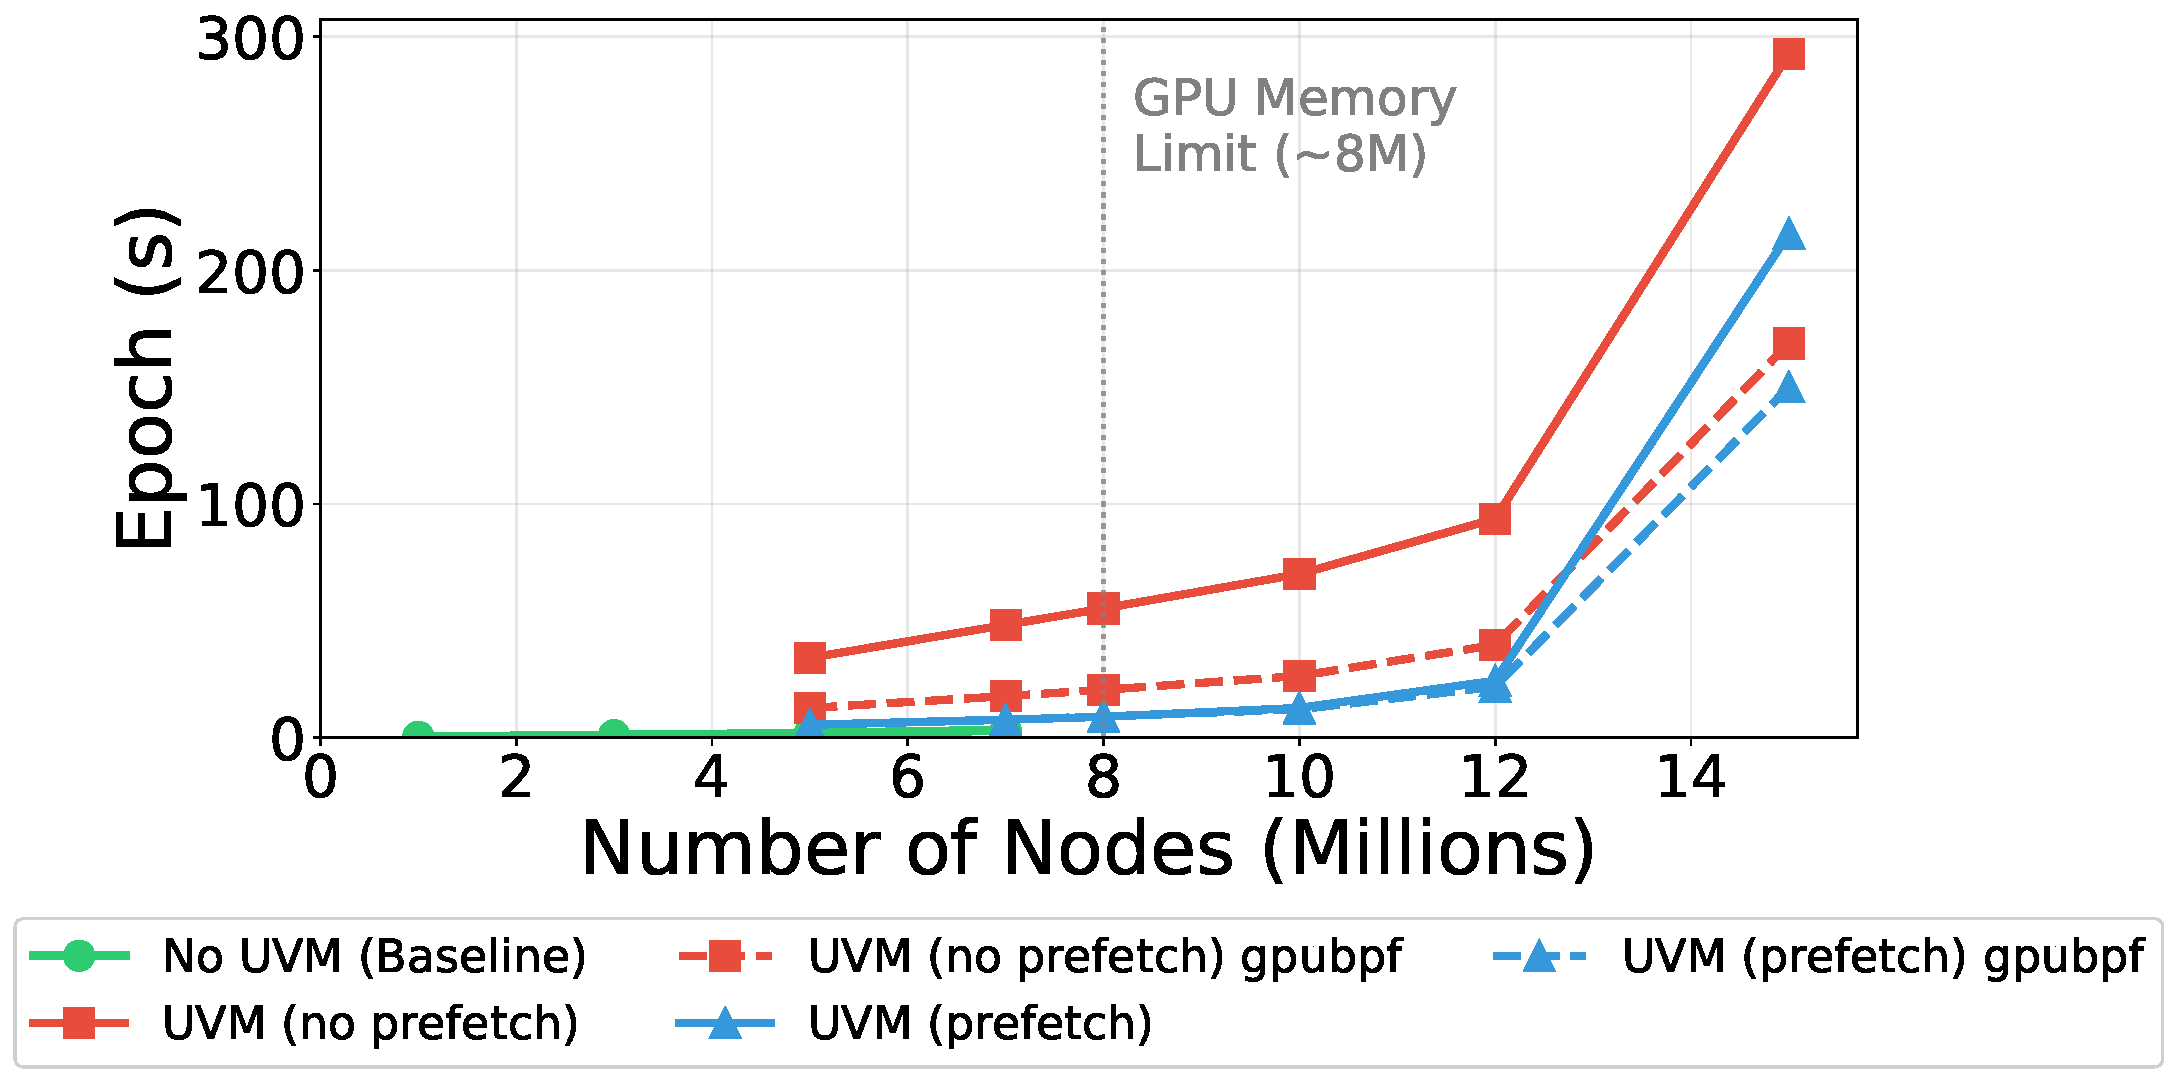
\includegraphics[width=\columnwidth]{img/results-raw/pytorch/uvm_benchmark_comparison.pdf}

\caption{GCN training epoch time vs graph size on PyTorch.}
% PyTorch 上 GCN 训练的单轮时间随图规模的变化。
\label{fig:gnn-epoch}
\end{figure}

\paragraph{Faiss Vector Search.}
% Faiss 向量检索。
We evaluate \sys on vector similarity search using the SIFT dataset with an IVF4096,Flat index, scaling from 20M (9.5GB) to 50M (24GB) and 100M (48GB, exceeding GPU memory).
% 我们使用 SIFT 数据集和 IVF4096,Flat 索引评估向量相似度检索，规模从 20M（9.5GB）到 50M（24GB）再到 100M（48GB，超过 GPU 显存）。
IVF indexes have a two-level structure: frequently-accessed centroids and larger posting lists, and Faiss operations have two distinct phases: BUILD performs sequential scans while SEARCH issues random accesses.
% IVF 索引具有两级结构：被频繁访问的聚类中心和更大的 posting list；Faiss 操作有两个不同阶段：BUILD 执行顺序扫描，SEARCH 发起随机访问。
\sys reduces build time by 21--29\% on 50M, scaling to 27--40\% on 100M as memory pressure grows.
% 在 50M 规模上，gpubpf 将构建时间降低 21--29\%，在 100M 上随内存压力增大扩大到 27--40\%。
For search workloads, \sys reduces latency by 10--16\% across different \texttt{nprobe} settings despite the random access patterns inherent in ANN search.
% 对于检索工作负载，尽管 ANN 检索固有的随机访问模式，gpubpf 在不同 \texttt{nprobe} 设置下仍将延迟降低 10--16\%。
As shown in \Cref{fig:faiss-perf}, the converged policy prefetches posting lists sequentially for oversubscribed datasets and uses stride prediction for K-means iterations during index construction; device-side eBPF programs also trigger prefetching of corresponding posting lists.
% 如 \Cref{fig:faiss-perf} 所示，收敛后的策略对超订数据集顺序预取 posting list，并在索引构建期间对 K-means 迭代使用步长预测；设备端 eBPF 程序还会触发相应 posting list 的预取。

The agent tested 8 policies over 5 iterations.
% 智能体在 5 轮迭代中测试了 8 个策略。
Initially, a momentum-based phase detector with cycle eviction improved BUILD but degraded SEARCH, as forward drift in search queries confused the detector.
% 最初，带周期驱逐的基于动量的阶段检测器改善了 BUILD 但恶化了 SEARCH，因为检索查询的前向漂移迷惑了检测器。
Fixing the classifier revealed eviction policy rather than phase detection controlled performance.
% 修正分类器后发现，控制性能的是驱逐策略而非阶段检测。
Version three, pairing the corrected detector with default eviction, converged.
% 第三个版本将修正后的检测器与默认驱逐配对，收敛成功。
A subsequent fast-path optimization introduced a state-machine bug (policy stuck in SEARCH mode), detected and fixed in one iteration.
% 随后的一项快速路径优化引入了一个状态机缺陷（策略卡在 SEARCH 模式），在一个迭代内被检出并修复。
Only 2 of 8 policies yielded positive results.
% 8 个策略中只有 2 个产生了正面结果。

\begin{figure}
\centering

\includegraphics[width=\columnwidth]{img/results-raw/faiss/faiss_benchmark_results.pdf}

\caption{Faiss index build time and query throughput under oversubscription.}
% 超订条件下 Faiss 索引构建时间与查询吞吐量。
\label{fig:faiss-perf}
\end{figure}

% Across all four case studies, \sys's programmable policies exploit workload structure (experts, KV-cache, graph structure, index layout) that existing UVM and framework-level mechanisms cannot leverage, and the agent's exploration followed a consistent pattern: broad initial policy, failure-driven refinement, and iterative convergence, with eBPF containment ensuring every failed attempt was recovered in seconds rather than requiring driver rebuilds or reboots.

\subsubsection{Multi-Tenant Memory, Bandwidth, and Scheduling}
% 多租户内存、带宽与调度
\label{sec:rq1-mt}

We evaluate \sys on multi-tenant GPU workloads, comparing per-tenant policies against global and framework-managed approaches.
% 我们在多租户 GPU 工作负载上评估 gpubpf，将每租户策略与全局策略和框架管理的方法进行对比。

\paragraph{Compute-bound Scheduler (LC + BE).}
% 计算密集型调度器（LC + BE）。
We evaluate \sys's eBPF struct\_ops scheduling policies on \emph{compute-bound} (SM-limited) multi-tenant workloads, without memory oversubscription.
% 我们在\emph{计算密集型}（SM 受限）的多租户工作负载上评估 gpubpf 基于 eBPF 的 struct\_ops 调度策略，不涉及内存超订。
2 latency-critical (LC) processes and 4 best-effort (BE) processes run concurrently, each with 4 CUDA streams submitting 50 compute kernels.
% 2 个延迟关键（LC）进程与 4 个尽力型（BE）进程并发运行，每个进程通过 4 条 CUDA 流提交 50 个计算内核。
We compare the native scheduler against \sys with differentiated timeslices (LC: 1s, BE: 200$\mu$s) using a preemption policy equivalent to GPREEMPT's~\cite{fan2025gpreempt} priority-based timeslice scheduling, implemented as a \sys eBPF program.
% 我们将原生调度器与采用差异化时间片的 gpubpf（LC：1 秒，BE：200$\mu$秒）对比，其抢占策略等价于 GPREEMPT~\cite{fan2025gpreempt} 的基于优先级的时间片调度，以 gpubpf eBPF 程序实现。
\Cref{fig:scheduler-latency} shows that \sys reduces LC P99 launch latency by 96\% (1188$\mu$s $\to$ 53$\mu$s).
% \Cref{fig:scheduler-latency} 显示，gpubpf 将 LC 的 P99 启动延迟降低 96\%（1188$\mu$秒 $\to$ 53$\mu$秒）。
BE throughput remains unchanged.
% BE 吞吐量保持不变。

\begin{figure}
\centering
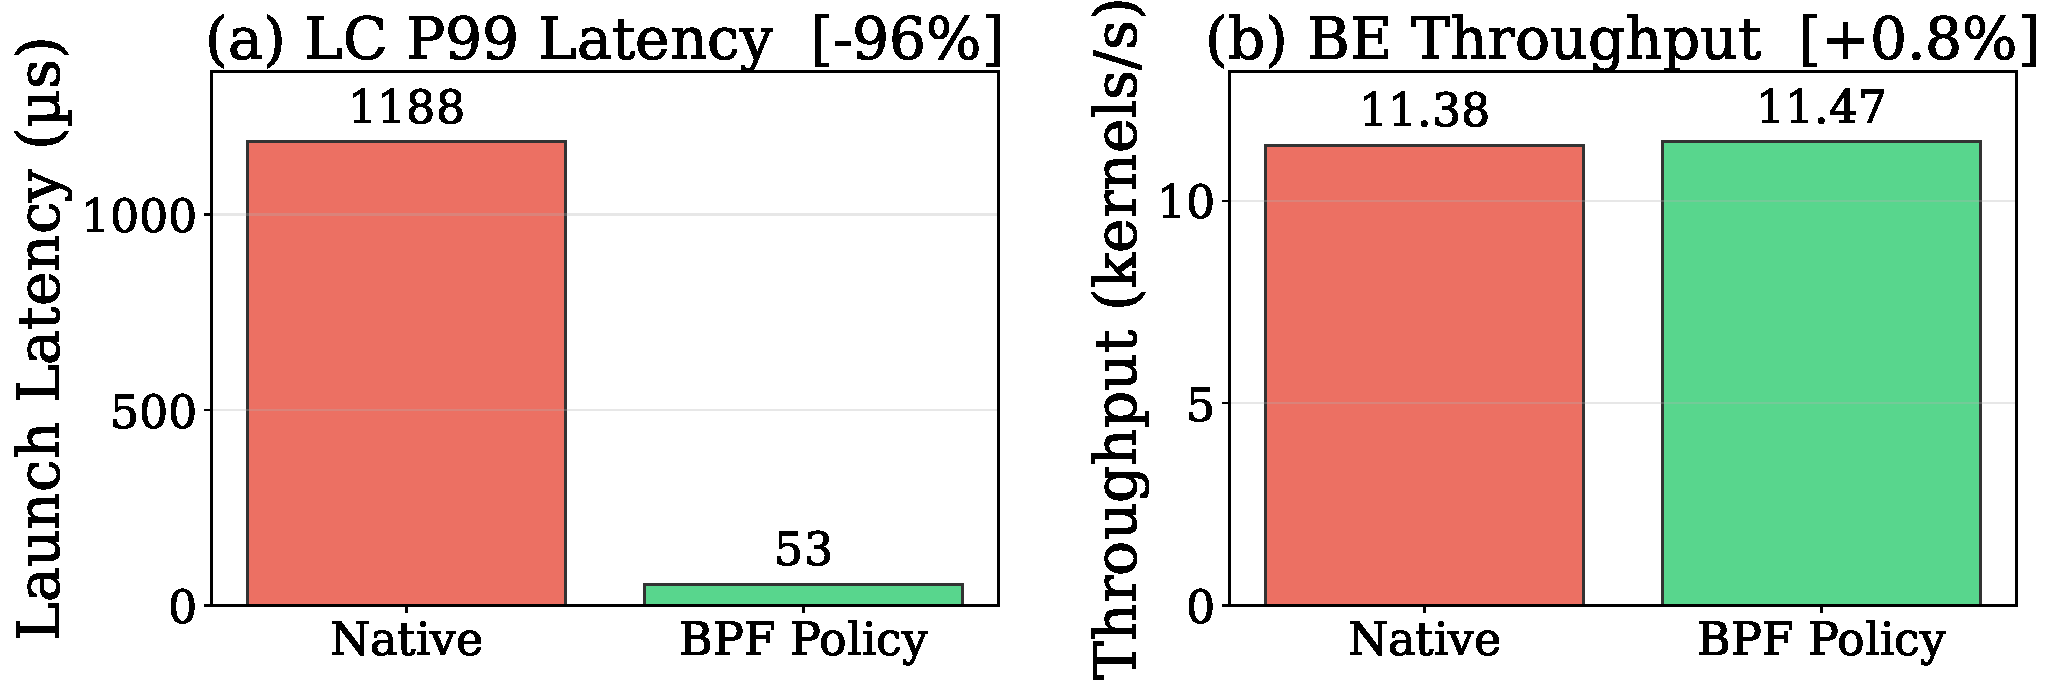
\includegraphics[width=\columnwidth]{img/results-raw/multi-tenant/scheduler_latency_throughput.pdf}

\caption{Multi-tenant GPU scheduling with \sys{} (LC: latency-critical, BE: best-effort).}
% 使用 gpubpf 的多租户 GPU 调度（LC：延迟关键型，BE：尽力型）。
\label{fig:scheduler-latency}
% \vspace{-1.5em}
\end{figure}

\paragraph{Memory-bound Priority Differentiation.}
% 内存密集型优先级区分。
We evaluate \sys's memory policies for priority differentiation on \emph{memory-bound} workloads under UVM oversubscription using HotSpot~\cite{che2009rodinia} (spatial locality), GEMM from PolyBench~\cite{grauer2012auto} (compute-intensive, memory-bound under UVM oversubscription), and K-Means~\cite{gu2020uvmbench} (sparse access).
% 我们在 UVM 超订下使用 HotSpot~\cite{che2009rodinia}（空间局部性）、来自 PolyBench~\cite{grauer2012auto} 的 GEMM（计算密集，在 UVM 超订下为内存受限）和 K-Means~\cite{gu2020uvmbench}（稀疏访问），在\emph{内存密集型}工作负载上评估 gpubpf 的内存优先级区分策略。
Each experiment runs two concurrent processes competing for GPU memory.
% 每个实验运行两个并发进程竞争 GPU 内存。
Policy labels use priority values 0--100 (lower = higher priority): \texttt{Prefetch(lo,hi)} prefetches pages for processes in that range, while \texttt{Evict(lo,hi)} selects eviction victims accordingly.
% 策略标签使用 0--100 的优先级数值（数值越低优先级越高）：\texttt{Prefetch(lo,hi)} 为处于该范围的进程预取页面，\texttt{Evict(lo,hi)} 则据此选择驱逐对象。
We compare against: (1)~no-policy execution, (2)~single-process runtime (Single~1$\times$), and (3)~theoretical optimum (2$\times$Single~1$\times$).
% 我们对比：(1) 无策略执行，(2) 单进程运行时（Single 1×），以及 (3) 理论最优（2×Single 1×）。

\Cref{fig:all-kernels-priority} shows that without policies, both processes degrade severely due to memory thrashing.
% \Cref{fig:all-kernels-priority} 显示，没有策略时，两个进程都因内存抖动而严重退化。
With \sys memory priority policies, total completion time improves by 55--92\%, and high-priority processes complete 6--19\% faster.
% 使用 gpubpf 内存优先级策略后，总完成时间改善 55--92\%，高优先级进程完成速度加快 6--19\%。
Critically, for these \emph{memory-bound} workloads, GPREEMPT-style~\cite{fan2025gpreempt} scheduler timeslice policies are \emph{ineffective} (<1\% improvement) because the bottleneck is UVM page faults and PCIe bandwidth, not GPU compute time.
% 关键在于，对于这些\emph{内存密集型}工作负载，GPREEMPT 式~\cite{fan2025gpreempt}调度器时间片策略\emph{无效}（改善不足 1\%），因为瓶颈是 UVM 缺页和 PCIe 带宽，而非 GPU 计算时间。
The scheduling results in \S\ref{sec:policy-mechanism} show the complementary case: timeslice policies improve latency when GPU compute is the bottleneck.
% \S\ref{sec:policy-mechanism} 的调度结果展示了互补情形：当 GPU 计算是瓶颈时，时间片策略能改善延迟。

\begin{figure}
\centering

\includegraphics[width=\columnwidth]{img/results-raw/multi-tenant/all_kernels_stacked.pdf}

\caption{Multi-tenant memory priority differentiation. Single 1$\times$: single-process time; 2$\times$Single 1$\times$: theoretical lower bound.}
% 多租户内存优先级区分。Single 1×：单进程时间；2×Single 1×：理论下界。
\label{fig:all-kernels-priority}
\end{figure}

\paragraph{Two-Tenant: High-Priority LLM Inference + Background Training.}
% 双租户：高优先级 LLM 推理 + 后台训练。
We run two tenants sharing a single GPU: T1 is a high-priority \texttt{llama.cpp} inference service (LC workload) serving 100 ShareGPT prompts at 0.2 RPS, and T2 is a background PyTorch GNN training job (BE workload) with 8M nodes requiring 36GB peak memory (oversubscribed).
% 我们让两个租户共享一块 GPU：T1 是高优先级的 \texttt{llama.cpp} 推理服务（LC 工作负载），以 0.2 RPS 服务 100 条 ShareGPT 提示；T2 是后台的 PyTorch GNN 训练作业（BE 工作负载），8M 节点，峰值内存需求 36GB（超订）。
We compare default UVM (driver FIFO/LRU) against \sys per-tenant memory and scheduler policies (combining Quota LRU, Tree-based Prefetch, and Dynamic Timeslice).
% 我们将默认 UVM（驱动 FIFO/LRU）与 gpubpf 的每租户内存和调度器策略（结合 Quota LRU、基于树的预取和动态时间片）进行对比。
\Cref{fig:two-tenant} shows mutual improvement: LC TPOT drops by 40--45\% and TTFT by 14--20\%, while GNN training simultaneously improves by 28\%, approaching the ideal fair share baseline.
% \Cref{fig:two-tenant} 显示双方同时受益：LC 的 TPOT 下降 40--45\%，TTFT 下降 14--20\%，同时 GNN 训练也改善 28\%，接近理想的公平份额基线。
This shows \sys reduces contention for both workloads rather than favoring one over the other.
% 这说明 gpubpf 减轻了两种工作负载之间的竞争，而非偏袒其中一方。

The tenants share an unpartitioned GPU managed by a system-wide policy.
% 租户共享一块由系统级策略管理的未分区 GPU。

\begin{figure}
\centering

\includegraphics[width=\columnwidth]{img/results-raw/multi-tenant/fig_colocated_results.pdf}

\caption{Two-tenant co-location: \texttt{llama.cpp} inference (LC) + GNN training (BE).}
% 双租户共置：\texttt{llama.cpp} 推理（LC）+ GNN 训练（BE）。
\label{fig:two-tenant}

\end{figure}

\begin{figure*}[!t]
\centering

\includegraphics[width=\textwidth]{img/results-raw/runtime/microbench_comparison.pdf}
\caption{Device-side overhead. (a) Naive per-thread injection vs \sys's SIMT-aware execution. (b) CPU map access latency via PCIe vs GPU-side operations.}
% 设备端开销。(a) 朴素的每线程注入与 gpubpf 的 SIMT 感知执行对比。(b) 经 PCIe 的 CPU map 访问延迟与 GPU 端操作对比。
\label{fig:microbench}
\end{figure*}

\subsubsection{Policies from Published Systems}
% 已发表系统的策略
\label{sec:policy-mechanism}

We evaluate whether \sys{} can express the policies of published state-of-the-art systems, and what the general mechanism costs when it runs the same policy as a native implementation.
% 我们评估 \sys{} 能否表达已发表最先进系统的策略，以及通用机制相对原生实现运行同一策略的开销。
\Cref{tab:published-policies} summarizes the seven policies, their execution requirements, and their implementations through \sys{}.
% \Cref{tab:published-policies} 汇总七种策略、其执行需求以及通过 \sys{} 实现的方式。

\begin{table*}[t]
\centering
\caption{Prior policies, their underlying mechanisms, and the \sys{} implementations evaluated in \Cref{fig:matched-ports}(a--g).}
% 既有策略、其底层机制以及 \Cref{fig:matched-ports}(a--g) 中评估的 \sys{} 实现。
\label{tab:published-policies}
\small
\setlength{\tabcolsep}{4pt}
\begin{tabularx}{\textwidth}{@{} >{\hsize=0.5\hsize\raggedright\arraybackslash}X >{\hsize=0.9\hsize\raggedright\arraybackslash}X >{\hsize=1.6\hsize\raggedright\arraybackslash}X @{}}
\toprule
System & Original policy & Original mechanism and \sys{} implementation \\
% 系统；原有策略；原有机制与 gpubpf 实现。
\midrule
MoE-Infinity~\cite{xue2025moeinfinity} & Match access predictions, rank expert prefetches, and select eviction victims. & A user-space runtime manages expert transfers; \sys{} implements cache decisions as host-side programs on the shared GPT-OSS-120B executor. \\
% MoE-Infinity：匹配访问预测、排列专家预取顺序并选择驱逐对象；用户态运行时管理专家传输，gpubpf 通过主机侧程序在共用 GPT-OSS-120B 执行器上实现缓存决策。
\addlinespace
Expert Buffering~\cite{huang2023towards} & Admit experts to the cache and prioritize eviction of experts unused by the current batch. & A user-space cache manages GPU buffers and CPU-to-GPU copies; \sys{} implements admission and eviction as host-side programs on the shared cache executor. \\
% Expert Buffering：决定专家缓存准入，优先驱逐当前批次不用的专家；用户态缓存管理 GPU 缓冲区和 CPU 到 GPU 的复制，gpubpf 通过主机侧程序在共用缓存执行器上实现准入与驱逐。
\addlinespace
FineMoE~\cite{yu2026finemoe} & Select a dynamic set of experts for speculative prefetch. & A user-space cache uses CUDA runtime transfers; \sys{} implements dynamic expert selection as a host-side program on the shared inference executor. \\
% FineMoE：动态选择推测预取的专家集合；用户态缓存通过 CUDA runtime 传输数据，gpubpf 通过主机侧程序在共用推理执行器上实现动态专家选择。
\addlinespace
Hummingbird~\cite{hu2026hummingbird} & Split background kernels to fill foreground idle intervals, with priority-aware memory management. & CUDA API interception and kernel splitting handle execution, while memory management modifies UVM; our host-side \sys{} port implements idle admission on the shared DNN executor. \\
% Hummingbird：拆分后台 GPU 内核以填充前台空闲区间，并按优先级管理内存；CUDA API 拦截与内核拆分负责执行，内存管理修改 UVM，我们的主机侧 gpubpf 移植在共用 DNN 执行器上实现空闲准入。
\addlinespace
POD-Attention~\cite{kamath2025pod} & Proportionally select prefill or decode work for each SM. & Native selection inside the GPU kernel becomes a device-side \sys{} program; the fused attention kernel executes the selected work. \\
% POD-Attention：按比例为各 SM 选择 prefill 或 decode 工作；GPU 内核中的原生选择逻辑由设备侧 gpubpf 程序实现，融合注意力内核执行所选工作。
\addlinespace
XSched~\cite{shen2025xsched} & Select the highest-priority task through preemptible command queues. & A user-space scheduler uses queue control and, at higher preemption levels, GPU instrumentation or driver interfaces; our host-side \sys{} port retains the original inter-kernel executor. \\
% XSched：通过可抢占命令队列选择最高优先级任务；用户态调度器控制队列，较高抢占级别还使用 GPU 插桩或驱动接口，我们的主机侧 gpubpf 移植保留原始内核间抢占执行器。
\addlinespace
GPREEMPT~\cite{fan2025gpreempt} & Control task admission and assign timeslices by priority. & User-space blocking/release relies on a modified GPU driver for timeslices; \sys{} implements these decisions with host- and driver-side programs on the same executor. \\
% GPREEMPT：控制任务准入并按优先级分配时间片；用户态阻塞与释放依赖修改后的 GPU 驱动控制时间片，gpubpf 通过主机侧和驱动侧程序在相同执行器上实现这些决策。
\bottomrule
\end{tabularx}
\end{table*}

\begin{figure*}[t]
\centering
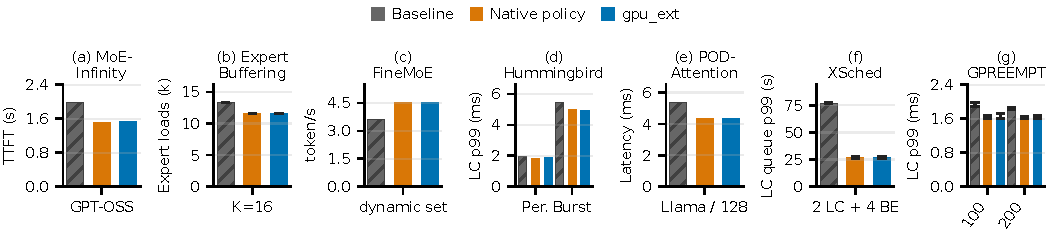
\includegraphics[width=\textwidth]{tex-revision/img/results-raw/revision/matched-policy-panels.pdf}
\caption{Policy comparisons on RTX~5090: workload baseline, native policy, and \sys on the same executor. Baselines are (a) prediction-disabled expert caching, (b) fixed-$K$ FIFO, (c) prefetching all positively predicted experts, (d,g) default scheduling, (e) two-stream FlashAttention, and (f) native CUDA. TTFT measures first-visible-text latency; panel (e) uses Llama decode batch 128. Bars show medians over five blocks, except (e) means and (f) ten blocks; whiskers in (b,f,g) show full ranges. Panel (d) uses idle admission; (g) uses VGG19 LC at 100 requests/s with ResNet152 BE at 100 or 200 requests/s.}
% RTX~5090 上的策略比较：相同执行器上的工作负载基线、原生策略与 gpubpf。基线为关闭预测的专家缓存（a）、固定 K 的 FIFO（b）、预取所有预测会用到的专家（c）、默认调度（d、g）、双流 FlashAttention（e）和原生 CUDA（f）。TTFT 表示首个可见文本延迟；面板（e）使用 Llama 解码批量 128。柱形为五组实验的中位数，但（e）为均值、（f）使用十组；（b、f、g）的须线表示完整范围。（d）使用空闲准入；（g）为每秒 100 个 VGG19 LC 请求，对应 ResNet152 BE 每秒 100 或 200 请求。
\label{fig:matched-ports}
\end{figure*}

\paragraph{Methodology}
% 方法
\Cref{fig:matched-ports} separates two comparisons: a workload baseline versus a native policy implementation measures policy benefit, while native versus \sys{} on the same executor measures the port's cost.
% \Cref{fig:matched-ports} 区分两层比较：工作负载基线与原生策略实现比较策略收益，相同执行器上的原生实现与 \sys{} 比较移植代价。
Each comparison pairs a native implementation with a \sys{} port of the same policy on the same workload and executor, on RTX~5090 (driver 575.57.08) with exclusive GPU access and repeated randomized trials.
% 每组对比在相同工作负载和执行器上，将原生实现与同一策略的 \sys{} 移植版配对，在 RTX~5090（驱动 575.57.08）上以独占 GPU 和重复随机试验运行。
Unless stated otherwise, we report medians with paired bootstrap intervals; POD's operator plot uses the mean of five per-run means.
% 除非另有说明，我们报告中位数及配对 bootstrap 区间；POD 算子图使用五次运行均值的平均值。

\paragraph{Results}
% 结果
With MoE-Infinity's policy, the native implementation and \sys{} reduce first-visible-text latency by 22.1\% and 22.5\%, respectively, relative to prediction-disabled expert caching across five paired runs.
% 采用 MoE-Infinity 策略时，五次配对运行中原生实现与 \sys{} 相比关闭预测的专家缓存，分别将首个可见文本延迟降低 22.1\% 和 22.5\%。
For Expert Buffering at the same cache capacity, both the native policy and \sys{} reduce whole-expert loads by 12.85\% relative to fixed-$K$ FIFO (\Cref{fig:matched-ports}(b)).
% 对 Expert Buffering，在相同缓存容量下，原生策略与 \sys{} 均相对固定 K 的 FIFO 将完整专家加载次数减少 12.85\%（\Cref{fig:matched-ports}(b)）。
With FineMoE's policy, \sys{} improves throughput by 24.6\% over a policy that prefetches every expert with a positive prediction; native and \sys{} throughput differ by 0.21\% in paired runs (95\% CI $[-0.17\%,+0.52\%]$).
% 采用 FineMoE 策略时，相比预取所有预测会用到的专家，\sys{} 将吞吐提高 24.6\%；原生与 \sys{} 在配对运行中的吞吐差异为 0.21\%（95\% CI $[-0.17\%,+0.52\%]$）。

With Hummingbird's policy, \sys{} lowers LC response p99 by 5.9--9.1\% relative to default scheduling across periodic and BurstGPT arrivals, compared with 7.5--8.2\% for the native policy.
% 采用 Hummingbird 策略时，在周期性和 BurstGPT 到达模式下，相对默认调度，\sys{} 将 LC 响应 p99 降低 5.9--9.1\%，原生策略降低 7.5--8.2\%。
For XSched with two LC and four BE processes, LC p99 latency from submission until the first thread block starts falls from 76.9~s under native CUDA to 27.0~s with the native policy and 27.3~s with \sys{} (\Cref{fig:matched-ports}(f)).
% 对 XSched，在两个 LC 和四个 BE 进程下，LC 从提交到首个线程块开始执行的 p99 延迟从原生 CUDA 的 76.9 秒降至原生策略的 27.0 秒和 \sys{} 的 27.3 秒（\Cref{fig:matched-ports}(f)）。
Under continuous background load, GPREEMPT's policy reduces LC response p99 from 1.796~ms under default scheduling to 1.615~ms with the native policy and 1.610~ms with \sys{}.
% 在连续后台负载下，GPREEMPT 策略将 LC 响应 p99 从默认调度的 1.796 毫秒降至原生策略的 1.615 毫秒和 \sys{} 的 1.610 毫秒。

For POD-Attention, we evaluate ten shapes over five blocks against non-fused FlashAttention and native POD implementations.
% 对 POD-Attention，我们在十种形状和五组实验中与未融合的 FlashAttention 及原生 POD 实现比较。
For Llama decode batch 128, operator latency falls from 5.360~ms with two-stream FlashAttention to 4.322~ms with the native policy and 4.344~ms with \sys{}.
% 在 Llama 解码批量 128 下，算子延迟从双流 FlashAttention 的 5.360 毫秒降至原生策略的 4.322 毫秒和 \sys{} 的 4.344 毫秒。

\paragraph{Mechanism cost}
% 机制代价
Expert Buffering incurs 0.7\% overhead; across ten shapes, POD's operator latency in paired runs decreases by up to 0.44\% or increases by up to 1.18\%.
% Expert Buffering 的开销为 0.7\%；在十种形状的配对运行中，POD 的算子延迟最多降低 0.44\% 或增加 1.18\%。
A UVM policy verified by the kernel incurs 3.2\% overhead with prefetch disabled in fifteen paired runs measuring page-fault handling.
% 在测量缺页处理的十五次配对运行中，通过内核验证的 UVM 策略在禁用预取时开销为 3.2\%。

\subsection{RQ2: Mechanism Cost}
% RQ2：机制代价
\label{sec:rq2-cost}

We measure hook, observability, and map-placement overheads below; \S\ref{sec:policy-mechanism} compares the execution costs of native and \sys{} implementations of the same policies.
% 下文测量钩子、可观测性和 map 放置开销；\S\ref{sec:policy-mechanism} 比较相同策略的原生实现与 \sys{} 实现的执行代价。

\paragraph{Verification Overhead.}
% 验证开销。
Load-time verification takes 141~ms for \texttt{kernelretsnoop} and 12~ms for \texttt{threadhist}.
% 加载时验证对 \texttt{kernelretsnoop} 耗时 141~ms，对 \texttt{threadhist} 耗时 12~ms。

\paragraph{Host Runtime Overhead.}
% 主机运行时开销。
We quantify the overhead of the \sys driver runtime independent of policy logic using GEMM from PolyBench~\cite{grauer2012auto} and HotSpot~\cite{che2009rodinia} (1.1$\times$ oversubscription, 35~GB working set) on RTX 5090.
% 我们使用 PolyBench~\cite{grauer2012auto} 的 GEMM 和 HotSpot~\cite{che2009rodinia}（1.1× 超订、35 GB 工作集）在 RTX 5090 上量化 gpubpf 驱动运行时独立于策略逻辑的开销。
With hooks enabled but no policy attached, the overhead is less than 0.2\%.
% 启用钩子但不附加策略时，开销小于 0.2\%。

\paragraph{Device-side Overhead.}
% 设备端开销。
We evaluate device-side observability tools built on \sys (\Cref{fig:obs-overhead}) using llama.cpp prefill on two GPUs: the P40 (Llama 1B, sequence-mixed) and the RTX~5090 (TinyLlama-1.1B, 512-token prefill with custom NVBit adapters~\cite{villa2019nvbit}).
% 我们在两块 GPU 上使用 llama.cpp 预填充评估基于 gpubpf 构建的设备端可观测工具（\Cref{fig:obs-overhead}）：P40（Llama 1B，序列混合）和 RTX~5090（TinyLlama-1.1B，512-token 预填充，定制 NVBit 适配器~\cite{villa2019nvbit}）。
Tools include \texttt{kernel\-ret\-snoop} (per-block finish timestamps), \texttt{thread\-hist} (load imbalance detection), and \texttt{launch\-late} (GPU kernel launch latency).
% 工具包括 \texttt{kernel\-ret\-snoop}（每块完成时间戳）、\texttt{thread\-hist}（负载不均衡检测）和 \texttt{launch\-late}（GPU 内核启动延迟）。
Overhead is measured as token/s degradation during prefill.
% 开销以预填充期间 token/s 的下降来衡量。
On the P40, \sys achieves 3--14\% overhead versus NVBit's 85--93\%, due to the warp-uniform execution model.
% 在 P40 上，得益于 warp 统一执行模型，gpubpf 的开销为 3--14\%，而 NVBit 为 85--93\%。
On the RTX~5090, \sys has lower overhead than NVBit for all three tools: 5.57\% versus 99.62\% for per-warp kernel-return logging, 2.97\% versus 10.35\% for the exit-count histogram, and 0.22\% versus 8.80\% for \texttt{launchlate}.
% 在 RTX~5090 上，gpubpf 在三个工具上的开销均低于 NVBit：逐 warp 内核返回记录为 5.57\% 对 99.62\%，退出计数直方图为 2.97\% 对 10.35\%，\texttt{launchlate} 为 0.22\% 对 8.80\%。
Attaching to a running process requires no application restart.
% 附加到正在运行的进程无需重启应用。

\begin{figure}[t]
\centering
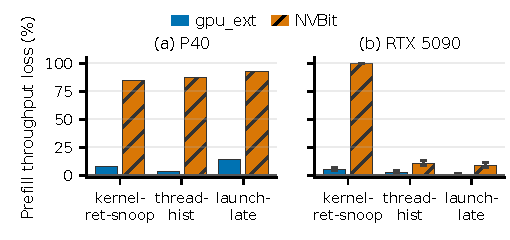
\includegraphics[width=\columnwidth]{tex-revision/img/results-raw/revision/obs-overhead-with-array.pdf}
\caption{Prefill throughput loss relative to an uninstrumented baseline. (a) P40, Llama 1B. (b) RTX~5090, TinyLlama-1.1B: ten baseline/tool pairs per configuration, except \sys kernelretsnoop (five independent pairs). Bars show means and whiskers show RTX~5090 run ranges; P40 uses original reported values. For \sys kernelretsnoop, records are collected after prefill (10.38\,ms, outside prefill timing).}
% 相对未插桩基线的预填充吞吐下降。(a) P40，Llama 1B。(b) RTX~5090，TinyLlama-1.1B：每个配置十组基线/工具配对，gpubpf kernelretsnoop 使用另外独立测量的五组配对。柱形为均值，须线为 RTX~5090 的运行范围；P40 使用原文报告值。gpubpf kernelretsnoop 在预填充后收集记录（10.38 ms，不计入预填充计时）。
\label{fig:obs-overhead}
\end{figure}

\paragraph{Device-side Runtime Optimization.}
% 设备端运行时优化。
We evaluate device-side \sys mechanisms using a vector-add CUDA GPU kernel (32 elements, 10K iterations) from cuda-sample~\cite{nvidia_cuda_samples} on RTX 5090.
% 我们使用来自 cuda-sample~\cite{nvidia_cuda_samples} 的 vector-add CUDA GPU 内核（32 个元素、10K 次迭代）在 RTX 5090 上评估 gpubpf 的设备端机制。
\Cref{fig:microbench}(a) compares \sys's SIMT-aware warp-level execution against eGPU~\cite{egpu} that injects eBPF bytecode without SIMT-specific verification and optimizations.
% \Cref{fig:microbench}(a) 将 gpubpf 的 SIMT 感知 warp 级执行与 eGPU~\cite{egpu} 对比，后者注入 eBPF 字节码而不进行面向 SIMT 的验证与优化。
The baseline incurs overhead due to per-thread execution and uncoalesced memory access, while \sys's warp-uniform execution and coalesced map access reduce overhead by 60--80\%.
% 基线因每线程执行和未合并的内存访问产生开销，而 gpubpf 的 warp 统一执行与合并 map 访问将开销降低 60--80\%。
\Cref{fig:microbench}(b) compares CPU map access via PCIe against GPU-side operations, motivating \sys's hierarchical map design that keeps hot state on GPU.
% \Cref{fig:microbench}(b) 对比了经 PCIe 的 CPU map 访问与 GPU 端操作，这促使 gpubpf 采用将热状态保留在 GPU 上的分层 map 设计。
We do not compare policy-level performance against the prior workshop version or Neutrino because they are limited to read-only observability (\S\ref{sec:background}). %\arq{Do we need this experimentation?  I guess you're wanting to show that this current version of the system is better than the workshop version, but I wonder if that is entirely surprising.}
% 我们不在策略层面与先前的工作坊版本或 Neutrino 比较，因为它们仅限于只读可观测性（\S\ref{sec:background}）。
